\documentclass[a4paper,12pt,twoside]{memoir}

% Castellano
\usepackage[spanish,es-tabla]{babel}
\selectlanguage{spanish}
\usepackage[utf8]{inputenc}
\usepackage[T1]{fontenc}
\usepackage{lmodern} % scalable font
\usepackage{microtype}
\usepackage{placeins}
\usepackage{eurosym}

\RequirePackage{booktabs}
\RequirePackage[table]{xcolor}
\RequirePackage{xtab}
\RequirePackage{multirow}

% Links
\usepackage[colorlinks]{hyperref}
\hypersetup{
	allcolors = {red}
}

% Ecuaciones
\usepackage{amsmath}

% Rutas de fichero / paquete
\newcommand{\ruta}[1]{{\sffamily #1}}

% Párrafos
\nonzeroparskip


% Imagenes
\usepackage{graphicx}
\newcommand{\imagen}[2]{
	\begin{figure}[!h]
		\centering
		\includegraphics[width=0.9\textwidth]{#1}
		\caption{#2}\label{fig:#1}
	\end{figure}
	\FloatBarrier
}

\newcommand{\imagenflotante}[2]{
	\begin{figure}%[!h]
		\centering
		\includegraphics[width=0.9\textwidth]{#1}
		\caption{#2}\label{fig:#1}
	\end{figure}
}



% El comando \figura nos permite insertar figuras comodamente, y utilizando
% siempre el mismo formato. Los parametros son:
% 1 -> Porcentaje del ancho de página que ocupará la figura (de 0 a 1)
% 2 --> Fichero de la imagen
% 3 --> Texto a pie de imagen
% 4 --> Etiqueta (label) para referencias
% 5 --> Opciones que queramos pasarle al \includegraphics
% 6 --> Opciones de posicionamiento a pasarle a \begin{figure}
\newcommand{\figuraConPosicion}[6]{%
  \setlength{\anchoFloat}{#1\textwidth}%
  \addtolength{\anchoFloat}{-4\fboxsep}%
  \setlength{\anchoFigura}{\anchoFloat}%
  \begin{figure}[#6]
    \begin{center}%
      \Ovalbox{%
        \begin{minipage}{\anchoFloat}%
          \begin{center}%
            \includegraphics[width=\anchoFigura,#5]{#2}%
            \caption{#3}%
            \label{#4}%
          \end{center}%
        \end{minipage}
      }%
    \end{center}%
  \end{figure}%
}

%
% Comando para incluir imágenes en formato apaisado (sin marco).
\newcommand{\figuraApaisadaSinMarco}[5]{%
  \begin{figure}%
    \begin{center}%
    \includegraphics[angle=90,height=#1\textheight,#5]{#2}%
    \caption{#3}%
    \label{#4}%
    \end{center}%
  \end{figure}%
}
% Para las tablas
\newcommand{\otoprule}{\midrule [\heavyrulewidth]}
%
% Nuevo comando para tablas pequeñas (menos de una página).
\newcommand{\tablaSmall}[5]{%
 \begin{table}
  \begin{center}
   \rowcolors {2}{gray!35}{}
   \begin{tabular}{#2}
    \toprule
    #4
    \otoprule
    #5
    \bottomrule
   \end{tabular}
   \caption{#1}
   \label{tabla:#3}
  \end{center}
 \end{table}
}

%
%Para el float H de tablaSmallSinColores
\usepackage{float}

%
% Nuevo comando para tablas pequeñas (menos de una página).
\newcommand{\tablaSmallSinColores}[5]{%
 \begin{table}[H]
  \begin{center}
   \begin{tabular}{#2}
    \toprule
    #4
    \otoprule
    #5
    \bottomrule
   \end{tabular}
   \caption{#1}
   \label{tabla:#3}
  \end{center}
 \end{table}
}

\newcommand{\tablaApaisadaSmall}[5]{%
\begin{landscape}
  \begin{table}
   \begin{center}
    \rowcolors {2}{gray!35}{}
    \begin{tabular}{#2}
     \toprule
     #4
     \otoprule
     #5
     \bottomrule
    \end{tabular}
    \caption{#1}
    \label{tabla:#3}
   \end{center}
  \end{table}
\end{landscape}
}

%
% Nuevo comando para tablas grandes con cabecera y filas alternas coloreadas en gris.
\newcommand{\tabla}[6]{%
  \begin{center}
    \tablefirsthead{
      \toprule
      #5
      \otoprule
    }
    \tablehead{
      \multicolumn{#3}{l}{\small\sl continúa desde la página anterior}\\
      \toprule
      #5
      \otoprule
    }
    \tabletail{
      \hline
      \multicolumn{#3}{r}{\small\sl continúa en la página siguiente}\\
    }
    \tablelasttail{
      \hline
    }
    \bottomcaption{#1}
    \rowcolors {2}{gray!35}{}
    \begin{xtabular}{#2}
      #6
      \bottomrule
    \end{xtabular}
    \label{tabla:#4}
  \end{center}
}

%
% Nuevo comando para tablas grandes con cabecera.
\newcommand{\tablaSinColores}[6]{%
  \begin{center}
    \tablefirsthead{
      \toprule
      #5
      \otoprule
    }
    \tablehead{
      \multicolumn{#3}{l}{\small\sl continúa desde la página anterior}\\
      \toprule
      #5
      \otoprule
    }
    \tabletail{
      \hline
      \multicolumn{#3}{r}{\small\sl continúa en la página siguiente}\\
    }
    \tablelasttail{
      \hline
    }
    \bottomcaption{#1}
    \begin{xtabular}{#2}
      #6
      \bottomrule
    \end{xtabular}
    \label{tabla:#4}
  \end{center}
}

%
% Nuevo comando para tablas grandes sin cabecera.
\newcommand{\tablaSinCabecera}[5]{%
  \begin{center}
    \tablefirsthead{
      \toprule
    }
    \tablehead{
      \multicolumn{#3}{l}{\small\sl continúa desde la página anterior}\\
      \hline
    }
    \tabletail{
      \hline
      \multicolumn{#3}{r}{\small\sl continúa en la página siguiente}\\
    }
    \tablelasttail{
      \hline
    }
    \bottomcaption{#1}
  \begin{xtabular}{#2}
    #5
   \bottomrule
  \end{xtabular}
  \label{tabla:#4}
  \end{center}
}



\definecolor{cgoLight}{HTML}{EEEEEE}
\definecolor{cgoExtralight}{HTML}{FFFFFF}

%
% Nuevo comando para tablas grandes sin cabecera.
\newcommand{\tablaSinCabeceraConBandas}[5]{%
  \begin{center}
    \tablefirsthead{
      \toprule
    }
    \tablehead{
      \multicolumn{#3}{l}{\small\sl continúa desde la página anterior}\\
      \hline
    }
    \tabletail{
      \hline
      \multicolumn{#3}{r}{\small\sl continúa en la página siguiente}\\
    }
    \tablelasttail{
      \hline
    }
    \bottomcaption{#1}
    \rowcolors[]{1}{cgoExtralight}{cgoLight}

  \begin{xtabular}{#2}
    #5
   \bottomrule
  \end{xtabular}
  \label{tabla:#4}
  \end{center}
}




\graphicspath{ {./img/} }

% Capítulos
\chapterstyle{bianchi}
\newcommand{\capitulo}[2]{
	\setcounter{chapter}{#1}
	\setcounter{section}{0}
	\chapter*{#2}
	\addcontentsline{toc}{chapter}{#2}
	\markboth{#2}{#2}
}

% Apéndices
\renewcommand{\appendixname}{Apéndice}
\renewcommand*\cftappendixname{\appendixname}

\newcommand{\apendice}[1]{
	%\renewcommand{\thechapter}{A}
	\chapter{#1}
}

\renewcommand*\cftappendixname{\appendixname\ }

% Formato de portada
\makeatletter
\usepackage{xcolor}
\newcommand{\tutor}[1]{\def\@tutor{#1}}
\newcommand{\course}[1]{\def\@course{#1}}
\definecolor{cpardoBox}{HTML}{E6E6FF}
\def\maketitle{
  \null
  \thispagestyle{empty}
  % Cabecera ----------------
\noindent
\includegraphics[width=\textwidth]{cabecera}\vspace{1cm}%
  \vfill
  % Título proyecto y escudo informática ----------------
  \colorbox{cpardoBox}{%
    \begin{minipage}{.8\textwidth}
      \vspace{.5cm}\Large
      \begin{center}
      \textbf{TFG del Grado en Ingeniería Informática}\vspace{.6cm}\\
      \textbf{\LARGE\@title{}}
      \end{center}
      \vspace{.2cm}
    \end{minipage}

  }%
  \hfill\begin{minipage}{.20\textwidth}
    
\includegraphics[width=\textwidth]{escudoInfor}
  \end{minipage}
  \vfill
  % Datos de alumno, curso y tutores ------------------
  \begin{center}%
  {%
    \noindent\LARGE
    Presentado por \@author{}\\ 
    en Universidad de Burgos --- \@date{}\\
    Tutor: \@tutor{}\\
  }%
  \end{center}%
  \null
  \cleardoublepage
  }
\makeatother


% Datos de portada
\title{Generación de rutas utilizando sistemas empotrados \\Documentación Técnica}
\author{Alejandro Fernández Lampreave}
\tutor{Dr. Alejandro Merino Gómez}
\date{\today}

\begin{document}

\maketitle



\cleardoublepage



%%%%%%%%%%%%%%%%%%%%%%%%%%%%%%%%%%%%%%%%%%%%%%%%%%%%%%%%%%%%%%%%%%%%%%%%%%%%%%%%%%%%%%%%



\frontmatter


\clearpage

% Indices
\tableofcontents

\clearpage

\listoffigures

\clearpage

\listoftables

\clearpage

\mainmatter

\appendix

\apendice{Plan de Proyecto Software}

\section{Introducción}
En este primer apartado de los anexos se encuentra toda la información sobre cómo se ha ido desarrollando en el tiempo el proyecto. De igual forma, un análisis sobre la viabilidad tanto económica como legal.

\section{Planificación temporal}
El trabajo de fin de grado se ha ido desarrollando a base de \textit{sprints} de 1 o 2 semanas de duración. Cada semana se hacía una revisión con el tutor de los objetivos que se habían marcado y dependiendo de si se habían alcanzado o no, se enfatizaba más sobre los mismos o se establecían nuevos objetivos. Algunas herramientas como ZenHub y GitHub han ayudado mucho en este proceso. En el GitHub del proyecto se pueden observar las diferentes fases por las que se ha ido pasando \url{https://github.com/alejandrolampreave/GPS}.

\subsection{Sprint 1 - 03/10/2018-10/10/2018}
La primera semana se dedica a repasar y profundizar sobre el funcionamiento de GitHub y a instalar e informarme sobre extensiones como ZenHub, para ello se ven diversos videotutoriales. Se realiza el primer \textit{issue} de prueba asociado al primer \textit{milestone}, me lo asigno a mi mismo y le pronostico una duración.

Además empiezo a configurar mi IDE siguiendo un tutorial a base de eclipse, librerías y plugins, pero se descubre que está obsoleto y nos decantamos por la instalación de Kinetis Design Studio que lo integra todo.

Podemos ver con más detalle en el Sprint 1 del repositorio, las diferentes actividades que se acometieron. 
Se calculó que tardaría 12 horas y al final se dedicaron 13 horas.

\subsection{Sprint 2 - 10/10/2018-17/10/2018}
La segunda semana se termina de instalar Kinetis y se realiza la primera práctica de Sistemas Empotrados, basada en un \textit{Hola Mundo} para familiarizarnos con el entorno de desarrollo. Una vez finalizada y ejecutada sin errores, el IDE se corrompe, no dejando cargar Processor Expert de ninguna de las maneras, quedando bloqueado.

Podemos ver con más detalle en el Sprint 2 del repositorio, las diferentes actividades que se acometieron. 
Se calculó que tardaría 9 horas y al final se dedicaron 16 horas.

\subsection{Sprint 3 - 17/10/2018-24/10/2018}
Los objetivos de este \textit{sprint} fueron arreglar Kinetis y documentarme sobre la comunicación entre el módulo GPS hacia la placa, para ello me leí el manual \textit{Adafruit Ultimate GPS Logger Shield}. Tras buscar mucha información por internet, hacer una reinstalación parcial de Processor Expert, reinstalar Kinetis desde cero, limpiar registros, configuraciones y parámetros, no se encuentra una solución definitiva, de forma que se opta por un formateo completo del ordenador. Además quedan soldadas las conexiones Digital I/O 0 y 1 con TX y RX respectivamente para transmitir los datos recogidos por el GPS a la placa.

Podemos ver con más detalle en el Sprint 3 del repositorio, las diferentes actividades que se acometieron. 
Se calculó que tardaría 45 horas y al final se dedicaron 50 horas.

\subsection{Sprint 4 - 24/10/2018-31/10/2018}
Una vez arreglado Kinetis, por fin se empieza con el proyecto en sí, el objetivo se marca en conseguir almacenar las coordenadas del acelerómetro en la tarjeta microSD. Después de instalar y configurar todos los componentes oportunos y de escribir el código, se consigue. Este \textit{sprint} será el primero que se mostrará en ZenHub pero los anteriores se pueden ver en GitHub.

Podemos ver con más detalle en el Sprint 4 del repositorio, las diferentes actividades que se acometieron. 
Se calculó que tardaría 21 horas y al final se dedicaron 30 horas.

\subsection{Sprint 5 - 07/11/2018-21/11/2018}
Primer \textit{sprint} que nos llevaría más de una semana, se plantea querer almacenar las coordenadas que arroja el GPS en la tarjeta microSD. Antes, las enviamos a la terminal Termite para ver qué muestra. 

Conseguiremos almacenar información en la tarjeta microSD pero no nos daremos cuenta hasta unos días más tarde que los datos son incompletos.

Podemos ver con más detalle en el Sprint 5 del repositorio, las diferentes actividades que se acometieron. 
Se calculó que tardaría 42 horas y al final se dedicaron 46 horas.

\subsection{Sprint 6 - 21/11/2018-28/11/2018 }
Esta fue la semana más caótica del proyecto, recién surgido el problema de la semana pasada se opta por avanzar sobre la funcionalidad de que solo se almacene información cuando se esté en movimiento gracias al acelerómetro. Reviso el manual del acelerómetro \textit{FXOS8700CQ} que incorpora la placa, sin obtener ninguna conclusión válida sobre esta funcionalidad.
Mientras tanto, sigo pensando cómo puedo solucionar el problema de la pérdida de información al escribir en la microSD.

Podemos ver con más detalle en el Sprint 6 del repositorio, las diferentes actividades que se acometieron. 
Se calculó que tardaría 2 horas y al final se dedicaron 10 horas.

\subsection{Sprint 7 - 28/11/2018-05/12/2018}
Finalmente, para tratar de arreglar la pérdida de caracteres, se opta por incluir en nuestro código un sistema operativo en tiempo real como \textit{FreeRTOS}, de forma que administre las diferentes tareas. Agregamos dos componentes nuevos y escribimos las tareas para así, lograr el objetivo.

Podemos ver con más detalle en el Sprint 7 del repositorio, las diferentes actividades que se acometieron. 
Se calculó que tardaría 45 horas y al final se dedicaron 50 horas.

\subsection{Sprint 8 - 05/12/2018-12/12/2018}
Esta semana fue un alto en el camino, se decidió avanzar bastante con la memoria, con la que se llevaba algo de retraso y actualizar el \textit{.gitIgnore} ya que estaba subiendo metadatos al repositorio.

Podemos ver con más detalle en el Sprint 8 del repositorio, las diferentes actividades que se acometieron. 
Se calculó que tardaría 22 horas y al final se dedicaron 26 horas.

\subsection{Sprint 9 - 12/12/2018-26/12/2018}
Durante estas dos semanas se elegirá la API con la que representaremos las coordenadas recogidas, finalmente nos decantamos por Mapbox y creamos una interfaz básica en html para poder probar nuestro fichero de coordenadas, después de convertirlo manualmente a la extensión \textit{GeoJSON}.

Podemos ver con más detalle en el Sprint 9 del repositorio, las diferentes actividades que se acometieron. 
Se calculó que tardaría 29 horas y al final se dedicaron 30 horas.

\subsection{Sprint 10 - 26/12/2018-09/01/2019}
Se fijó como objetivo que la conversión entre NMEA y GeoJSON fuera transparente al usuario, había varias opciones pero finalmente se optó por ayudarnos de Mygeodata por una cuestión de tiempo, haciendo una petición a través de un \textit{script} de Python.

Podemos ver con más detalle en el Sprint 10 del repositorio, las diferentes actividades que se acometieron. 
Se calculó que tardaría 8 horas y al final se dedicaron 20 horas. 

\subsection{Sprint 11 - 09/01/2019-16/01/2019}
Ahora que la conversión del fichero funcionaba de forma óptima, era hora de juntar todo, se habilitó la subida de archivos al servidor, conseguimos ejecutar la conversión de forma autónoma y se descomprimió el directorio que generaba MyGeoData, para poder acceder al archivo convertido y representarlo en el mapa. Además se acometieron algunos cambios en la interfaz de la página.

Podemos ver con más detalle en el Sprint 11 del repositorio, las diferentes actividades que se acometieron. 
Se calculó que tardaría 7 horas y al final se dedicaron 15 horas.

\subsection{Sprint 12 - 16/01/2019-23/01/2019}
En este \textit{sprint} se decidió que debíamos implementar alguna mejora en el código ya fuera de manera gráfica o alguna funcionalidad nueva. Conseguimos fechar los archivos subidos, añadimos el botón de ``Descargar imagen'' y el de ``Centrar mapa en mi posición'', intentamos \textit{hostear} la página, finalizamos la memoria y empezamos los anexos.

Podemos ver con más detalle en el Sprint 12 del repositorio, las diferentes actividades que se acometieron. 
Se calculó que tardaría 10 horas y al final se dedicaron 11 horas.

\subsection{Sprint 13 - 23/01/2019-30/01/2019}
Esta semana la dedicamos a avanzar en los anexos, crear la máquina virtual con la configuración necesaria para el correcto visionado de la página web y añadimos a nuestra interfaz una plantilla HTML para que fuera más atractiva al usuario.

Podemos ver con más detalle en el Sprint 13 del repositorio, las diferentes actividades que se acometieron. 
Se calculó que tardaría 29 horas y se cumplió con la estimación.

\subsection{Sprint 14 - 30/01/2019-06/02/2019}
El objetivo primordial fue habilitar el acelerómetro para la detección de movimiento y en caso de no detectarlo, pausar el registro de coordenadas en la tarjeta microSD para no almacenar información de forma redundante. Además terminaremos los anexos y comprobaremos la calidad del código con Sonarcloud.

Podemos ver con más detalle en el Sprint 14 del repositorio, las diferentes actividades que se acometieron. 
Se calculó que tardaría 29 horas y se cumplió la estimación.

\subsection{Sprint 15 - 06/02/2019-13/02/2019}
Incorporamos excepciones al código, se hicieron los test para las pruebas del sistema, subimos los instaladores del proyecto y grabamos la ruta que se entrega con el proyecto.

Podemos ver con más detalle en el Sprint 15 del repositorio, las diferentes actividades que se acometieron. 
Se calculó que tardaría 16 horas y al final se dedicaron 15 horas.

\section{Estudio de viabilidad}
En este apartado se hará el análisis sobre la viabilidad económica y legal del proyecto.

\subsection{Viabilidad económica}

\subsubsection{Coste de personal}
Vamos a calcular el coste de tener a un programador a sueldo a lo largo de 18 semanas, o lo que es lo mismo 4 meses y medio. Promediando 22 horas a la semana a un precio por hora de 9\euro  , el sueldo es el que se muestra:
\begin{table}[ht!]
\centering
\begin{tabular}{l}
\rowcolor[HTML]{EFEFEF} 
\multicolumn{1}{c}{\cellcolor[HTML]{EFEFEF}\textbf{Salario mensual}} \\
22 horas\/ semana * 4 semanas * 15\euro \/ hora = 1320\euro            
\end{tabular}
\caption{Salario mensual}
\label{CosteMensual}
\end{table}

A esos 1320\euro  habría que sumarle los abonos a la seguridad social por parte de la empresa, en nuestro caso un 23.60\% por contingencias comunes, un 1.35\% por AT y EP (Accidente de Trabajo y Enfermedad Profesional), un 5.50\% por desempleo y un 0.60 por formación. \cite{seguridadsocial} Hace un total de 31.05\%. 

\begin{table}[ht!]
\centering
\label{my-label}
\begin{tabular}{ll}
Salario mensual          	& 1.320\euro    \\
Seguridad Social (31.05\%) 	& 409,86\euro  \\ \hline
Coste mensual            	& 1.729,86\euro \\
Por 4 meses y medio         &             \\ \hline
\textbf{Coste total del personal}     & 7.784,37\euro 
\end{tabular}
\caption{Coste total del personal.}
\end{table}

\subsubsection{Coste de hardware}
Para desarrollar el proyecto se ha hecho uso de un porátil con un Intel Core i3 M370, una Nvidia GeForce 315M, disco duro sólido de 240GB y 8GB de memoria RAM con un coste total de 700\euro . Consideraremos una vida útil de 7 años, por lo que el coste amortizado para 4 meses y medio son 37.5\euro .
Calculemos ahora el coste total del hardware sumando la placa de desarrollo,el módulo GPS y la tarjeta microSD:
\begin{table}[ht!]
\centering
\label{my-label}
\begin{tabular}{ll}
Portatil coste amortizado    				& 37,5\euro  \\
Placa de desarrollo FRDM-K64F \cite{placa} 	& 32,52\euro \\
Ultimate GPS logger shield \cite{gps}      	& 39,06\euro \\ 
Tarjeta microSD 16gb 				     	& 3,9\euro 	 \\ \hline
\textbf{Coste total} 						& 112,98\euro
\end{tabular}
\caption{Coste total del hardware.}
\end{table}

\subsubsection{Otros costes}
Tendremos en consideración otros gastos como internet:

Fibra óptica simétrica 42\euro /mes x 4 meses y medio = 189\euro

\subsubsection{Coste total}
Por lo tanto el coste total del proyecto sumando todas las cantidades anteriores es de:
\begin{table}[ht!]
\centering
\label{my-label}
\begin{tabular}{ll}
Coste de personal    & 7.784,37\euro \\
Coste de hardware    & 112,98\euro   \\
Otros costes         & 189\euro      \\ \hline
\textbf{Coste total} & 8.086,35\euro
\end{tabular}
\caption{Coste total del proyecto.}
\end{table}

\subsubsection{Beneficios}
Una vez calculados los gastos por desarrollar el proyecto es hora de calcular los posibles beneficios de la venta del proyecto o bien de su explotación. Teniendo en cuenta que los costes han rondado los 8.000\euro , con que hubiera un comprador dispuesto a ofrecer 12.000\euro  y sacar 4.000\euro  de beneficios nos daríamos por satisfechos.

El sistema está orientado a toda la población en general que tenga intención de registrar una ruta, ya sea gente deportista o del mundo del motor, como también jefes a empleados en una flota de vehículos o padres controladores desconfiados de sus hijos y viceversa.

Aparte de la venta, también podría interesarnos un sistema de suscripciones al servicio de forma que, o bien compraran ellos el \textit{hardware} o se lo alquilamos y pagan por el derecho de ingresar a la página y subir sus ficheros de coordenadas. 

A un precio de 20\euro  mensuales por suscripción, con 34 personas suscritas durante 1 año conseguiríamos recuperar todo el dinero invertido. 

Sin duda es un riesgo asumible teniendo en cuenta que el coste del proyecto no es muy elevado y los ingresos pueden dispararse a corto medio plazo. Ideal para inversores con no mucho capital, dispuestos a arriesgar y con opciones a disparar sus beneficios.

\subsection{Viabilidad legal}
Hablando desde el punto de vista de la viabilidad legal del proyecto, éste se encuentra bajo una licencia de tipo, ``GNU General Public License v3.0'' la cual permite el uso comercial, la modificación, su distribución, el uso privado y el uso de patentes. Evitando así cualquier tipo de responsabilidad y garantía. \cite{gpslicense}

Si hablamos de los términos de uso de Mapbox expresan de forma clara que no debes vender su código a terceros pero no hay problema si tu aplicación lo integra para dar servicio a tus propios usuarios finales. \cite{mapbox}

La plantilla HTML que hemos incluido\cite{pagina} en nuestro proyecto cuenta con la licencia MIT (Massachusetts Institute of Technology), cuya única condición es que se distribuya la licencia original con todas las copias del software que se hagan.

Por último Mygeodata recalca que no debes reproducir, duplicar, vender o utilizar sus servicios si lo vas a hacer con mala intención. \cite{mygeodata}

\apendice{Especificación de Requisitos}

\section{Introducción}
En este apartado se incluyen los objetivos y requisitos marcados al inicio, entre el alumno y el tutor para el proyecto.
De manera adicional, se han añadido algunos no establecidos al inicio pero que se han considerado pertinentes a lo largo del desarrollo.

\section{Objetivos generales}
El desarrollo de este proyecto tiene el objetivo de desentramar la cadena NMEA aportada por el módulo GPS adherido a la placa de desarrollo FRDM-K64F, almacenar los mensajes NMEA en la tarjeta microSD activándose con el movimiento y conseguir mostrar en un mapa la ruta seguida por el usuario.

\section{Catálogo de requisitos}
En esta sección detallaremos los requisitos funcionales y no funcionales del proyecto.

\subsection{Requisitos funcionales}
\begin{itemize}
\tightlist
\item
    \textbf{RF1-Conexión del GPS:} El GPS debe establecer conexión satelital.
\item
    \textbf{RF2-Almacenar las coordenadas:} La placa guarda la información en la tarjeta.
\item
    \textbf{RF3-Almacenamiento de archivos NMEA:} Subir el archivo del usuario al servidor.
\item
    \textbf{RF4-Conversión de archivos:} Transformar el archivo NMEA a uno con extensión GeoJSON.
\item
    \textbf{RF5-Descompresión del fichero:} Descomprimir el fichero generado por MyGeoData.
\item
	\textbf{RF6-Mostrar mapa:} Representa en un mapa las coordenadas del fichero.
\item
    \textbf{RF7-Geolocalizar posición:} Geolocaliza tu posición y centra el mapa en donde estés.
\item
    \textbf{RF8-Descargar mapa:} Descarga el mapa que se visualice en ese momento como una imagen PNG.
\item
    \textbf{RF9-Modificar vista del mapa:} Añade o quita zoom, rota el mapa sobre su eje o cambia de vista.
\item  
    \textbf{RF10-Mensaje de error:} En caso de subir un fichero no admitido se mostrará un mensaje de error con el motivo.
\end{itemize}

\subsection{Requisitos no funcionales}
\begin{itemize}
\tightlist
\item
    \textbf{RNF1-Usabilidad:} El usuario debe sentirse familiarizado con la interfaz y ésta ha de ser \textit{user friendly}. Además debe ser \textit{responsive design} de forma que la web se amolde a las diferentes pantallas. 
\item
    \textbf{RNF2-Eficiencia:} tanto el módulo GPS almacenando coordenadas, como la web mostrando la ruta, deben tener el menor tiempo de respuesta posible.
\item
    \textbf{RNF3-Escalabilidad:} El proyecto debe ser escalable para que se puedan aumentar sus funcionalidades de forma rápida y sencilla.
\item
    \textbf{RNF4-Mantenibilidad:} Deben proporcionarse mejoras y mantenimiento de forma periódica.
\item
    \textbf{RNF5-Confiabilidad:} El proyecto ha de realizar las funciones para las que fue creado obteniendo los resultados esperados.
\item
    \textbf{RNF6-Disponibilidad:} La aplicación debe estar disponible el máximo tiempo posible, minimizando posibles caídas temporales del sistema.
\end{itemize}

\clearpage
\section{Especificación de requisitos}

\begin{table}[ht!]
\centering
\begin{tabular}{|
>{\columncolor[HTML]{EFEFEF}}l |p{0.8\linewidth}|}
\hline
\textbf{RF 1}            & \cellcolor[HTML]{EFEFEF}\textbf{Conexión del GPS.}                                                                   \\ \hline
\textbf{Descripción}     & El GPS debe establecer conexión satelital. \\ \hline
\textbf{Precondiciones}  & A la placa de desarrollo se le suministra corriente.\\ \hline
\textbf{Acciones}        & El módulo GPS busca comunicación con los satélites.\\ \hline
\textbf{Postcondiciones} & El GPS transmite su posición 1 vez por segundo.                   \\ \hline
\textbf{Importancia}     & Alta.                                                                                                                  \\ \hline
\end{tabular}
\caption{RF1 - Conexión del GPS.}
\label{RF1}
\end{table}

\begin{table}[ht!]
\centering
\begin{tabular}{|
>{\columncolor[HTML]{EFEFEF}}l |p{0.8\linewidth}|}
\hline
\textbf{RF 2}            & \cellcolor[HTML]{EFEFEF}\textbf{Almacenar las coordenadas.}                                                                   \\ \hline
\textbf{Descripción}     & La placa guarda la información en la tarjeta. \\ \hline
\textbf{Precondiciones}  & Se ha inicializado el sistema de almacenamiento y hay una tarjeta introducida.\\ \hline
\textbf{Acciones}        & La placa comienza a escribir en la tarjeta microSD.\\ \hline
\textbf{Postcondiciones} & Obtenemos un fichero con los mensajes NMEA transmitidos por el GPS. \\ \hline
\textbf{Importancia}     & Alta.                                                                                                                  \\ \hline
\end{tabular}
\caption{RF2 - Almacenar las coordenadas.}
\label{RF2}
\end{table}

%%se sube el archivo a temporal, se le pone fecha, se mueve, se convierte, se almacena la conversión.
\begin{table}[ht!]
\centering
\begin{tabular}{|
>{\columncolor[HTML]{EFEFEF}}l |p{0.8\linewidth}|}
\hline
\textbf{RF 3}            & \cellcolor[HTML]{EFEFEF}\textbf{Almacenamiento de archivos NMEA.}                                                                   \\ \hline
\textbf{Descripción}     & Subir el archivo del usuario al servidor. \\ \hline
\textbf{Precondiciones}  & El usuario selecciona el archivo que quiere subir.\\ \hline
\textbf{Acciones}        & El archivo es enviado a una carpeta temporal y es movido a ``subidas''.\\ \hline
\textbf{Postcondiciones} & Queda almacenado el archivo. \\ \hline
\textbf{Importancia}     & Alta.                                                                                                                   \\ \hline   
\end{tabular}
\caption{RF3 - Almacenamiento de archivos NMEA.}
\label{RF3}
\end{table}

\begin{table}[ht!]
\centering
\begin{tabular}{|
>{\columncolor[HTML]{EFEFEF}}l |p{0.8\linewidth}|}
\hline
\textbf{RF 4}            & \cellcolor[HTML]{EFEFEF}\textbf{Conversión de archivos.}                                                                   \\ \hline
\textbf{Descripción}     & Transformar el archivo NMEA a uno con extensión GeoJSON. \\ \hline
\textbf{Precondiciones}  & El usuario debe seleccionar un archivo local y subirlo.\\ \hline
\textbf{Acciones}        & Se ejecuta el script en Python de la API de MyGeoData.\\ \hline
\textbf{Postcondiciones} & Se genera un fichero con extensión zip. \\ \hline
\textbf{Importancia}     & Alta.                                                                                                                   \\ \hline   
\end{tabular}
\caption{RF4 - Conversión de archivos.}
\label{RF4}
\end{table}

\begin{table}[ht!]
\centering
\begin{tabular}{|
>{\columncolor[HTML]{EFEFEF}}l |p{0.8\linewidth}|}
\hline
\textbf{RF 5}            & \cellcolor[HTML]{EFEFEF}\textbf{Descompresión del fichero.}                                                                   \\ \hline
\textbf{Descripción}     & Descomprimir el fichero generado por MyGeoData. \\ \hline
\textbf{Precondiciones}  & Debe existir el fichero comprimido de MyGeoData.\\ \hline
\textbf{Acciones}        & Se descomprime el fichero.\\ \hline
\textbf{Postcondiciones} & Aparecen los archivos descomprimidos dentro de una carpeta. \\ \hline
\textbf{Importancia}     & Alta.                                                                                                                   \\ \hline   
\end{tabular}
\caption{RF5 - Descompresión del fichero.}
\label{RF5}
\end{table}

\begin{table}[ht!]
\centering
\begin{tabular}{|
>{\columncolor[HTML]{EFEFEF}}l |p{0.8\linewidth}|}
\hline
\textbf{RF 6}            & \cellcolor[HTML]{EFEFEF}\textbf{Mostrar mapa.}                                                                   \\ \hline
\textbf{Descripción}     & Representa en un mapa las coordenadas del fichero. \\ \hline
\textbf{Precondiciones}  & Disponer de un archivo en formato GeoJSON.\\ \hline
\textbf{Acciones}        & La API de Mapbox utiliza ese archivo.\\ \hline
\textbf{Postcondiciones} & Se representa un mapa con la ruta. \\ \hline
\textbf{Importancia}     & Alta.                                                                                                                   \\ \hline   
\end{tabular}
\caption{RF6 - Mostrar mapa.}
\label{RF6}
\end{table}

\begin{table}[ht!]
\centering
\begin{tabular}{|
>{\columncolor[HTML]{EFEFEF}}l |p{0.8\linewidth}|}
\hline
\textbf{RF 7}            & \cellcolor[HTML]{EFEFEF}\textbf{Geolocalizar posición.}                                                                   \\ \hline
\textbf{Descripción}     & Geolocaliza tu posición y centra el mapa en donde estés. \\ \hline
\textbf{Precondiciones}  & El mapa debe estar parcialmente cargado.\\ \hline
\textbf{Acciones}        & El usuario selecciona ``Centrar en mi posición''.\\ \hline
\textbf{Postcondiciones} & Se obtiene un mapa centrado en tu posición actual. \\ \hline
\textbf{Importancia}     & Baja.                                                                                                                   \\ \hline   
\end{tabular}
\caption{RF7 - Geolocalizar posición.}
\label{RF7}
\end{table}

\begin{table}[ht!]
\centering
\begin{tabular}{|
>{\columncolor[HTML]{EFEFEF}}l |p{0.8\linewidth}|}
\hline
\textbf{RF 8}            & \cellcolor[HTML]{EFEFEF}\textbf{Descargar mapa.}                                                                   \\ \hline
\textbf{Descripción}     & Descarga el mapa que se visualice en ese momento como una imagen PNG. \\ \hline
\textbf{Precondiciones}  & El mapa debe estar cargado por completo.\\ \hline
\textbf{Acciones}        & El usuario selecciona ``Descargar mapa''.\\ \hline
\textbf{Postcondiciones} & Se inicia la descarga del mapa. \\ \hline
\textbf{Importancia}     & Baja.                                                                                                                   \\ \hline   
\end{tabular}
\caption{RF8 - Descargar mapa.}
\label{RF8}
\end{table}

\begin{table}[ht!]
\centering
\begin{tabular}{|
>{\columncolor[HTML]{EFEFEF}}l |p{0.8\linewidth}|}
\hline
\textbf{RF 9}            & \cellcolor[HTML]{EFEFEF}\textbf{Modificar vista del mapa.}                                                                   \\ \hline
\textbf{Descripción}     & Añade o quita zoom, rota el mapa sobre su eje o cambia de vista. \\ \hline
\textbf{Precondiciones}  & El mapa debe estar parcialmente cargado.\\ \hline
\textbf{Acciones}        & El usuario selecciona algún botón de modificación del mapa de la vista actual o se desplaza a través de él.\\ \hline
\textbf{Postcondiciones} & Se obtiene un mapa con diferente vista. \\ \hline
\textbf{Importancia}     & Baja.                                                                                                                   \\ \hline   
\end{tabular}
\caption{RF9 - Modificar vista del mapa.}
\label{RF9}
\end{table}

\begin{table}[ht!]
\centering
\begin{tabular}{|
>{\columncolor[HTML]{EFEFEF}}l |p{0.8\linewidth}|}
\hline
\textbf{RF 10}            & \cellcolor[HTML]{EFEFEF}\textbf{Mensaje de error.}                                                                   \\ \hline
\textbf{Descripción}     & En caso de subir un fichero no admitido se mostrará un mensaje de error con el motivo. \\ \hline
\textbf{Precondiciones}  & Haber seleccionado un fichero para subir.\\ \hline
\textbf{Acciones}        & El usuario presiona ``Subir archivo''.\\ \hline
\textbf{Postcondiciones} & De ser un fichero inválido saltará una alerta explicando el motivo. \\ \hline
\textbf{Importancia}     & Media.                                                                                                                   \\ \hline   
\end{tabular}
\caption{RF10 - Mensaje de error.}
\label{RF10}
\end{table}

\clearpage
\section{Diagrama de casos de uso}
En esta sección mostraremos el diagrama de casos de uso de nuestra aplicación.
\imagen{casodeuso.PNG}{Diagrama de casos de uso del proyecto}
\apendice{Especificación de diseño}

\section{Introducción}
En esta sección detallaremos el diseño procedimental y el arquitectónico.

\section{Diseño procedimental}
En este apartado veremos el diseño interno del proyecto, especificando los detalles de los diferentes algoritmos. En este caso nos vamos a ayudar de un diagrama de secuencias que explicará el caso más completo que se podría dar en el proyecto.
\begin{figure}[!h]
	\centering
	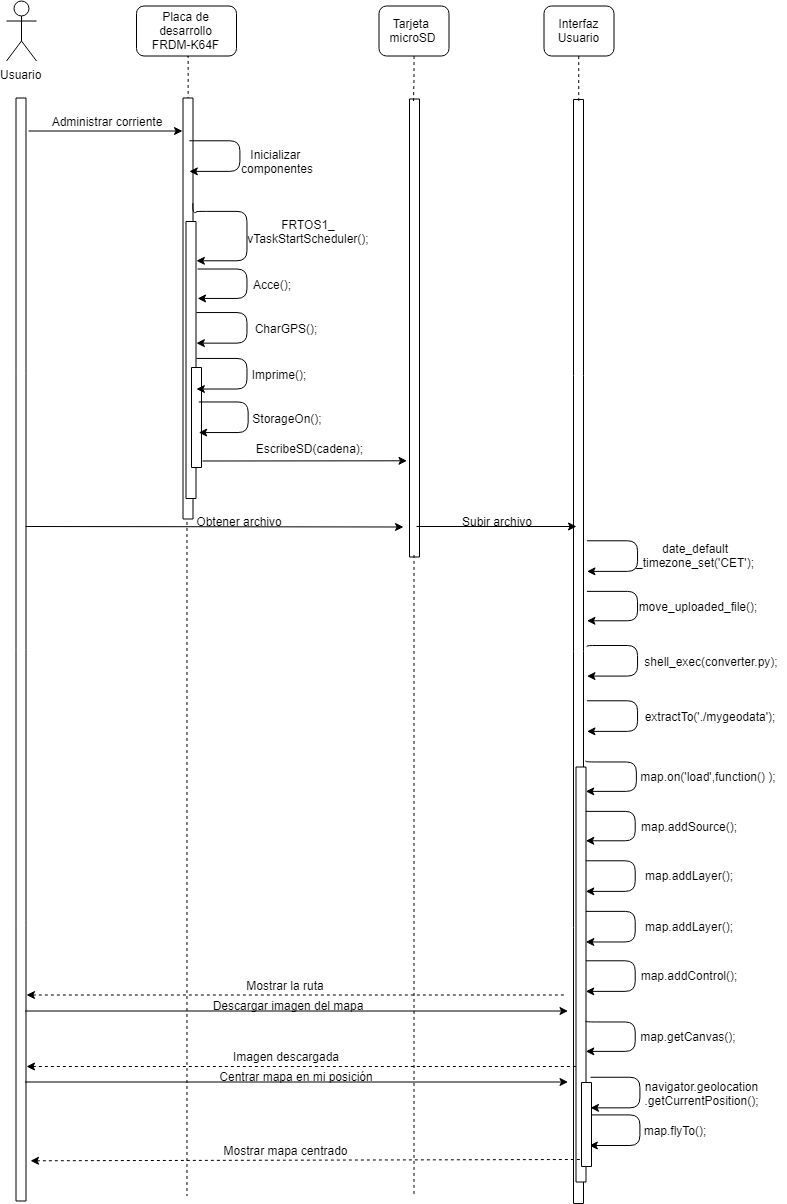
\includegraphics[width=1\textwidth]{diagramasecuencia.PNG}
	\caption{Diagrama de secuencias del proyecto.}\label{fig:diagramasecuencia.PNG}
\end{figure}
\FloatBarrier

\section{Diseño arquitectónico}
En esta sección veremos como se relacionan los diferentes módulos. Desglosaremos el diseño arquitectónico en dos secciones ya que contamos con dos partes claramente diferenciadas.

\subsection{Sistema operativo a tiempo real (RTOS)}
La arquitectura de programación utilizada en el funcionamiento de la placa de desarrollo es comúnmente denominada como ``Sistema operativo a tiempo real'' o RTOS \cite{arquitectura}. Usada en proyectos donde la complejidad es alta y es imprescindible la inclusión de requerimientos de tiempo real, el sistema operativo se encarga de decidir en que momento se debe ejecutar cada tarea a través de interrupciones también autogestionadas. En nuestro caso distinguimos las tareas de almacenar en la cadena los datos enviados por el GPS, la de comprobar los valores del acelerómetro para parar la escritura de datos en caso necesario y la de imprimir los caracteres de la cadena. 

En cuanto se le transmite corriente a la placa, ejecuta el código que alberga en la memoria flash, inicializa los componentes, las tareas y por último, el sistema operativo de tiempo real que las administra.
\imagen{arquitectura.PNG}{Diagrama básico de la arquitectura RTOS.\cite{arquitectura}}

\subsection{Modelo Vista Controlador}
El patrón utilizado para la interfaz web ha sido MVC\cite{mvc}. Se trata de uno de los diseños más usados y separa la vista respecto a la lógica de la aplicación. Intervienen en este diseño 3 componentes:
\begin{itemize}
\tightlist
\item
    \textbf{Modelo:} Se encarga de los datos y maneja la información con la que funciona el proyecto. También conocida como lógica de negocio. En nuestro caso se trata de la API de Mapbox y la de MyGeoData.
\item
    \textbf{Vista:} Se trata de la interfaz, la parte más visible a través de la cual el usuario solicita las acciones y donde se muestra la información. Nuestra página web cumpliría con esta misión mostrando los datos, en este caso la ruta del usuario en el mapa de la forma que él ha especificado.
\item
    \textbf{Controlador:} Es el intermediario entre los dos anteriores, recoge las peticiones del usuario para pasárselas al modelo y devuelve la información a la vista que ha transmitido éste. En nuestro proyecto cobra un papel relevante al ser el encargado de recoger el archivo al usuario, convertirlo y pasárselo al modelo con la configuración solicitada, para que éste después nos devuelva la información que debe ser mostrada en base a los datos aportados.
\end{itemize}
\imagen{mvc.PNG}{Comportamiento de los 3 componentes.\cite{mvcimg}}







\apendice{Dossier técnico de programación}

\section{Introducción}
En este manual vamos a detallar de la forma más precisa posible, cómo reanudar este proyecto para que se pueda seguir con el desarrollo si así se desea.

\section{Estructura de directorios}
Este proyecto se encuentra con la siguiente distribución de carpetas:
\begin{itemize}
	\item
	\textbf{src:} se encuentra todo el código de la aplicación.
	\item
	\textbf{src/Interface:} contiene el código de la interfaz, tanto la página web como el convertidor y algunos ficheros de ejemplo.
	\item
	\textbf{src/Interface/subidas:} aloja los archivos subidos a la página web.
	\item
	\textbf{src/Interface/mygeodata:} almacena los archivos convertidos a GeoJSON y descomprimidos.
	\item
	\textbf{src/DattaLogger:} contiene el código que lleva incorporada la placa de desarrollo, encargado de almacenar las coordenadas en función del movimiento. 
	\item
	\textbf{Documentación:} nos encontramos con los PDF de la memoria y anexos, los archivos de \textit{latex} y las imágenes.
	\item
	\textbf{Selenium Test:} contiene los test creados con Selenium IDE para la interfaz.
	\item
	\textbf{Instalables:} contiene un link a todos los ejecutables que se han necesitado en el proyecto. (\textit{Kinetis}, \textit{Termite}, \textit{Python} y \textit{XAMPP}).
\end{itemize}

\section{Manual del programador}
\subsection{Instalación Kinetis Design Studio}
La primera parte del proyecto (la de la placa GPS) se ha desarrollado con la última versión de Kinetis (3.2.0) disponible en la página web oficial de NXP .
A continuación se aporta el enlace con la última versión:

\href{https://nxp.flexnetoperations.com/control/frse/product?entitlementId=402114997&lineNum=1&authContactId=115669057&authPartyId=124808297} {\texttt{https://nxp.flexnetoperations.com/control/frse/product...}}

\subsection{Instalación de Termite}
La terminal utilizada para visualizar los datos recogidos por la placa de desarrollo ha sido Termite en su versión 3.4 \textit{(complete setup)}. En el siguiente enlace encontraremos la última versión de Termite.

\url{https://www.compuphase.com/software_termite.htm}

\subsection{Instalación de Python}
Para poder ejecutar el archivo de conversión de forma local necesitaremos Python en nuestro ordenador. En este caso ha sido utilizado Python 3.7.0.
En el siguiente enlace podemos encontrar la última versión de Python disponible.

\href{http://www.oracle.com/technetwork/java/javase/downloads/javafxscenebuilder-1x-archive-2199384.html}{\texttt{http://www.oracle.com/technetwork/java/javase/downloads...}}

\subsection{Instalación de XAMPP}
Para poder ejecutar nuestra página en nuestro ordenador necesitaremos emular un servidor local, para lo que he utilizado XAMPP. Para  Además necesitaremos hacer algunos ajustes de configuración para que reconozca archivos Python (extensión .py). Voy a indicar el directorio por defecto, pero cada uno tendrá que ir a su directorio de instalación. 
\begin{itemize}
\tightlist
\item
	En el archivo de configuración C:\textbackslash{}xampp\textbackslash{}apache\textbackslash{}conf\textbackslash{}httpd.conf añadir la extensión .py en la línea del \textit{AddHandler} de forma que quede: AddHandler cgi-script .cgi .pl .asp .py
\item
	En la línea \textit{Options Indexes FollowSymLinks} debe tener la configuración \textit{ExecCGI}.
\item
	La primera línea de script de python debe ser la ruta a python.
\item
	Por último debemos reiniciar XAMPP para que se apliquen los cambios.
\end{itemize}

\imagen{configapache.PNG}{Cambios necesarios en los archivos de configuración sobre el manejador.}

\imagen{configapache2.PNG}{Inclusión de ExecCGI en las opciones.}

Para la ejecución local, debemos meter la carpeta \textit{interface} del proyecto en la carpeta de XAMPP \textit{htdocs}, en mi caso: \textit{C:\textbackslash{}xampp\textbackslash{}htdocs}
 
A continuación se encuentra el enlace a la página de Apache donde podremos descargar la última versión de XAMPP:
\url{https://www.apachefriends.org/es/download.html}

\section{Compilación, instalación y ejecución}

\subsection{Importar el proyecto en Kinetis}
Debemos descargar el proyecto exportado comprimido y subido a GitHub que contiene no solo el código fuente si no todos los componentes y la configuración: \url{https://github.com/alejandrolampreave/GPS}.
A continuación lo descomprimimos y ya podemos importarlo en Kinetis.

Para importar en Kinetis hacemos clic en \textit{File > Import}. Seguidamente seleccionamos la opción \textit{Existing Projects into Workspace} y seleccionamos la carpeta descomprimida. 
\imagen{import.PNG}{File>Import para importar nuestro proyecto a Kinetis.}

\imagen{import2.PNG}{Seleccionamos ``Existing Projects into Workspace''.}

%\begin{figure}[!h]
%	\centering
%	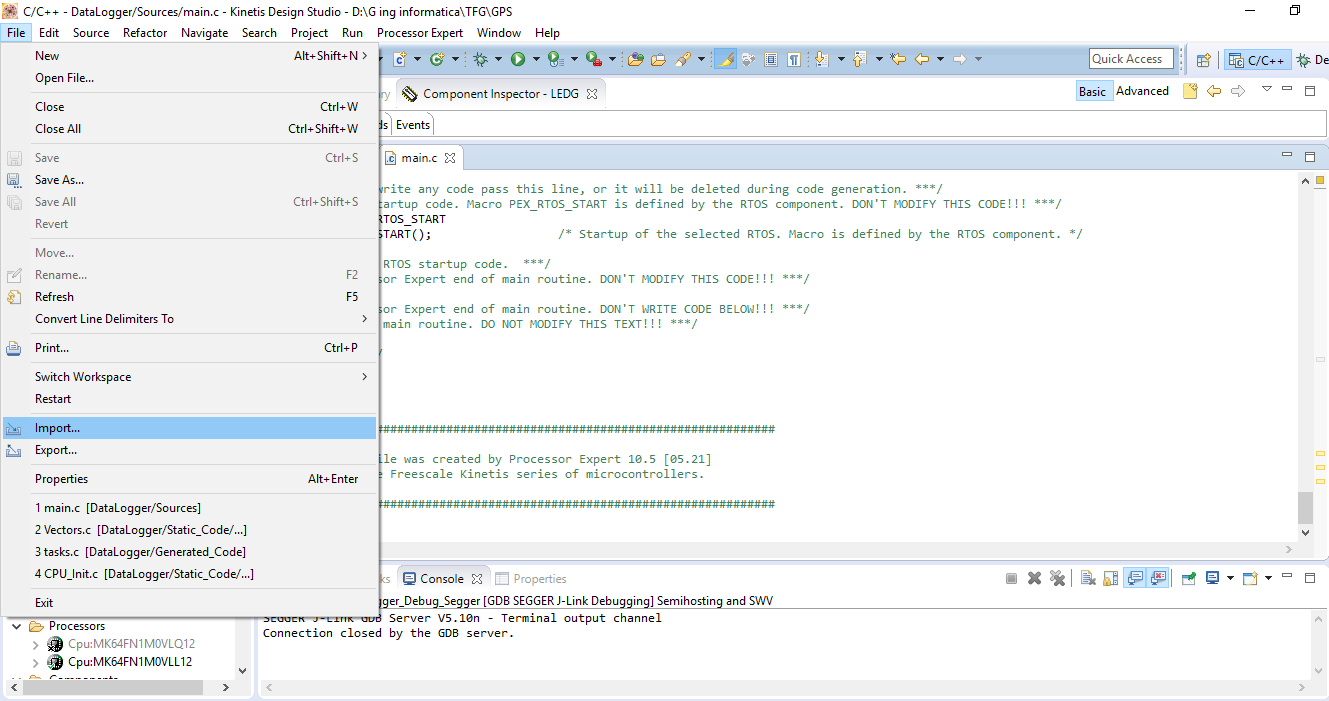
\includegraphics[width=0.8\textwidth, height=11.5cm]{import.PNG}
%	\caption{Importamos el proyecto a nuestro \textit{workspace} de .}\label{fig:import.png}
%\end{figure}
%\FloatBarrier
Ya podríamos empezar a trabajar en el proyecto.

\subsection{Grabar el programa en la placa}
Para grabar el programa en la placa de desarrollo tan solo debemos conectar la placa de desarrollo al conector de la placa de desarrollo OpenSDA y ejecutar nuestro programa dando al \textit{Run}, observando que la memoria seleccionada en ese momento sea la \textit{flash} y no la RAM.
\imagen{run.PNG}{Ejecutamos el programa para que quede almacenado en la memoria \textit{Flash} de la placa.}

\subsection{Ejecución}
Por último para ejecutar, solo tendremos que iniciar el servicio de Apache de XAMPP, abrir el navegador e introducir la siguiente url: \url{http://localhost/interface/index.html} para que se nos muestre la página de inicio de forma local. Una vez cargada podremos subir nuestro archivo, recogido por nuestro GPS y almacenado en la tarjeta microSD, para que se nos muestre en el mapa la ruta que hayamos hecho.
\imagen{apache.PNG}{Iniciamos el servicio de Apache.}

\section{Pruebas del sistema y calidad del código}
A lo largo de todo el desarrollo del proyecto se ha ido probando todo lo que se iba añadiendo para asegurarnos que no se perdiera ninguna funcionalidad a medida que avanzábamos. En caso de que diera algún error o algo no saliera según lo esperado, se replanteaba lo que se quería implementar y se buscaban posibles soluciones dentro de la misma opción o se pensaba en una alternativa válida.

Tanto desde el punto de vista del usuario como para nosotros mismos se habilitó el \textit{led} rgb de la placa de forma que nos indicase en todo momento qué estaba haciendo, \textit{led} verde obtención de coordenadas, \textit{led} rojo escritura en tarjeta. Además se ha comprobado que únicamente se permita la subida de archivos con extensión .txt, que es como se almacenan en la tarjeta.

De forma adicional se ha hecho uso de la herramienta de Selenium IDE, con la cual se ha desarrollado un pequeño test que comprobase la carga de los diferentes bloques de la página, incluyendo el mapa final. Se adjuntan los test junto con el proyecto.
\imagen{test.PNG}{Test realizado mediante Selenium IDE.}

En la última fase del proyecto se realizó una prueba en un ambiente real, dentro de un coche con la placa de desarrollo, para que registrara la ruta. Luego se introdujo la tarjeta en el ordenador y se subió a la página web, mostrando de forma satisfactoria la ruta seguida.

En cuanto a la calidad del código se refiere barajamos varias herramientas, entre ellas: SonarQube, Codacy, CodeClimate y CodeBeat. Finalmente seleccionamos SonarQube por ser una de las más importantes y que mejor se adaptaba al proyecto. En su página web seleccionamos el método \textit{online}, nos redireccionó a una página llamada Sonarcloud y tras descargarnos el ``sonar-scanner-3.3.0.1492'' ejecutamos un comando que nos dieron para generar el análisis. Cabe destacar que solo hemos podido pasar el escáner a los archivos de la interfaz, ya que al pasar el \textit{build wraper} proporcionado por la herramienta por nuestros ficheros fuentes en C no los reconocía. Diría que es porque la \textit{Build Tool} utilizado en Kinetis no es GCC si no uno específico llamado \textit{Cross ARM GCC}. 

Obtuvimos buenos resultados pero tras unas pequeñas mejoras, incluyendo algunas de la plantilla HTML utilizada, conseguimos mejorar la calidad de nuestro código sustancialmente. Algunos de los errores fueron marcados como falsos positivos, pero fueron acompañados por una explicación en tal caso. El link para comprobar la calidad del código es: \url{https://sonarcloud.io/dashboard?id=alejandrolampreave_GPS}
\imagen{sonarcloud1.PNG}{Escaneo realizado antes de corregir el código.}
\imagen{sonarcloud2.PNG}{Escaneo realizado tras corregir la mayoría de errores.}




\apendice{Documentación de usuario}

\section{Introducción}
Vamos a explicar cómo grabar una ruta con la placa GPS, así como la subida del fichero generado a la web para poder visualizarla en el mapa.
\section{Requisitos de usuarios}
Para poder registrar una ruta necesitamos:
\begin{itemize}
	\item
	Disponer de una placa de desarrollo FRDM-K64F con un módulo GPS incorporado y cableado como se ha detallado en la memoria.
    \item
    Tener grabada en su memoria flash (como se entrega) el programa que le va a permitir almacenar las coordenadas.
    \item
    Disponer de un ordenador con una correcta instalación de XAMPP y Python (dado que no está \textit{hosteada}).
    \item
    Un navegador instalado y conexión a internet.
    \item
    Una tarjeta microSD.
    \item
    Un soporte \textit{hardware} que permita leer tarjetas microSD.
\end{itemize}

\section{Instalación}
El proyecto, propiamente dicho, no requiere ser instalado previamente en un ordenador para funcionar, dado que se trata de una página web y la placa GPS va con el programa incorporado, pero sí se debe haber hecho una correcta configuración previa, como ya se ha hecho referencia. 

\section{Manual del usuario}
Una vez que está todo correctamente configurado, solo queda poder utilizar el proyecto. Para ello vamos a dividirlo en dos partes claramente diferenciadas.
\subsection{Grabar la ruta}
Debemos suministrar corriente a la placa de desarrollo, para lo cual utilizaremos una batería externa conectada por micro USB, que nos brinda máxima movilidad. Debemos esperar a que consiga conexión con los satélites, el led \textit{fix} rojo lo indicará cuando deje de parpadear de forma constante, y lo haga cada 3 segundos aproximadamente. 

Se recomienda que el módulo GPS esté lo menos cubierto posible, ya que ayudará a su rápida conexión, de no ser así podría tardar hasta media hora. Se recuerda que en caso de necesidad se le podría acoplar una antena GPS externa, que le otorga mejor conexión. Ahora solo queda empezar a moverse y automáticamente se empezarán a almacenar las coordenadas, el led rojo será en encargado de indicar que se están almacenando las coordenadas correctamente en la tarjeta microSD. En caso de detenerse se parará el almacenamiento, para una mayor eficiencia.

\subsection{Mostrar la ruta}
Una vez finalizada la ruta, simplemente debemos extraer la tarjeta microSD de la placa e introducirla a nuestro ordenador. Veremos un archivo llamado ``LOG\_GPS\_NMEA.txt'' ese será nuestro archivo, abrimos la página web, \url{http://localhost/interface/index.html} y daremos a ``Seleccionar archivo'', escogeremos nuestro archivo y seleccionaremos ``Subir archivo''.

De forma automática nuestras coordenadas serán almacenadas en el directorio \textit{/subidas}, las convertirá a formato GeoJSON y las almacenará en \textit{/mygeodata} y se mostrará la ruta en el mapa.
\imagen{subir.PNG}{Página principal donde subiremos los archivos.}

\subsection{Información de la página}
A modo informativo se nos muestra una serie de cajas con información sobre el proyecto. Así como de presentación para posibles nuevos usuarios.
\imagen{web1.PNG}{Características generales de la página y funcionalidad básica.}
\imagen{web2.PNG}{Herramientas del mapa y opción a GPS.}
\imagen{web3.PNG}{Opiniones y preguntas.}

\subsection{Opciones de la interfaz}
Se nos presentan algunas herramientas en la ventana donde se muestra la ruta. La primera ``Centrar en mi posición'', te saltará una solicitud para poder detectar tu posición, tras aceptarla, el mapa se centrará en tu localización. También tienes la opción de moverte por el mapa, tienes a tu disposición unos controles a la derecha para poder añadir o quitar zoom y volver a orientarte hacia el norte. Además, podemos descargar la imagen con la ruta en alta resolución si seleccionamos ``Descargar imagen''.

Seleccionando con el botón derecho del ratón se nos permite cambiar en ángulo de visión del mapa y rotarlo. De esta forma podemos visualizar los edificios en 3D.
\imagen{3D.PNG}{Edificios en 3D tras haber cambiado la vista.}



\bibliographystyle{plain}
\bibliography{bibliografiaAnexos}

\end{document}
